\documentclass[11pt,a4paper]{article}
\usepackage{gtu-el-yazisi}
\begin{document}
\notbilgi{Alan Teorisi}{Uygulama 7 (vize sonrası) -- Eş merkezli küre/silindir yüzeyler}{Uygulama-7-Vize-sonrasi.pdf}
% yerel yardımcı: üstü çizili (sadeleştirilen) terimler
\newcommand\iptalX[3]{\tikz[baseline=(c.base)]{\node[inner sep=0pt](c){$#2#3$};\draw[#1,line width=0.5pt](c.south west)--(c.north east);}}
\newcommand\iptalK[2]{\iptalX{murekkep}{#1}{#2}}
\newcommand\iptalO[2]{\iptalX{turuncukalem}{#1}{#2}}
\newcommand\iptal[1]{\mathpalette\iptalK{#1}}
\newcommand\iptalt[1]{\mathpalette\iptalO{#1}}

\sayfa{1}
\noindent\textbf{1)}\quad
\begin{minipage}[c]{0.36\linewidth}
\centering
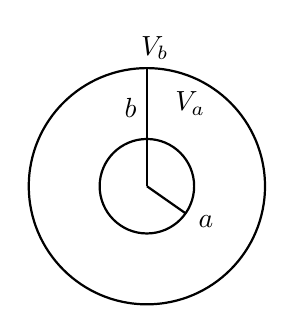
\begin{tikzpicture}[line width=0.8pt]
  \draw (0,0) circle (1.5);
  \draw (0,0) circle (0.6);
  \draw (0,0) -- (0,1.5);
  \draw (0,0) -- (-35:0.6);
  \node[left] at (0,1.0) {$b$};
  \node at (0.1,1.75) {$V_b$};
  \node at (0.55,1.05) {$V_a$};
  \node at (0.75,-0.45) {$a$};
\end{tikzpicture}
\end{minipage}\hfill
\begin{minipage}[c]{0.58\linewidth}
$a<r<b$ \quad $V(r)=\dfrac{V_a-V_b}{\frac1a-\frac1b}\,\dfrac1r+\dfrac{aV_a-bV_b}{a-b}$

\medskip
$r<a$ \quad $\vec E=0$ \quad $\vec E=-\mathrm{grad}\,V$

$V(r)=C$ \quad $V(a)=V_a=C$

\medskip
\hfill $\kutula{V(r)=V_a}$\hfill\null
\end{minipage}

\medskip
\noindent $r>b$ \qquad $\Delta V=0$ \qquad
$\iptal{\dfrac{1}{r^2}}\,\dfrac{\partial}{\partial r}\Bigl(r^2\dfrac{\partial V}{\partial r}\Bigr)=0$
\[ r^2\frac{\partial V}{\partial r}=A \quad\Rightarrow\quad V(r)=\frac{A}{r}+B \]
\[ r\to\infty:\quad V(r)=0\ \text{olmalıdır}\ \Rightarrow\ B=0 \]
\[ r=b:\quad V(b)=V_b=\frac{A}{b}\ \Rightarrow\ A=bV_b \]
\[ V(r)=\frac{bV_b}{r} \]

\medskip\hrule\medskip
\[ a<r<b:\quad \vec E=-\mathrm{grad}\,V=\frac{V_a-V_b}{\frac1a-\frac1b}\,\frac{1}{r^2}\,\vec e_r \]
\[ r<a:\quad \vec E=0 \]
\[ r>b:\quad \vec E=-\mathrm{grad}\,V=-\frac{\partial}{\partial r}\Bigl(\frac{bV_b}{r}\Bigr)\vec e_r=\frac{bV_b}{r^2}\,\vec e_r \]
\begin{align*}
r=a:\quad \vec E &= \frac{\vec E^{+}(a)+\vec E^{-}(a)}{2} \\
&= \frac12\left[\frac{V_a-V_b}{\frac1a-\frac1b}\,\frac{1}{a^2}\right]\vec e_r \\
&= \frac12\,\frac{b}{a}\left[\frac{V_a-V_b}{b-a}\right]\vec e_r
\end{align*}

\sayfa{2}
\noindent
\begin{minipage}[t]{0.34\linewidth}
$d\vec F=\rho_s\,ds\,\vec E$
\end{minipage}\hfill
\begin{minipage}[t]{0.62\linewidth}
$ds=a^2\sin\theta\,d\phi\,d\theta$ \\
$\mathrm{div}\,\vec D=\rho_s$ \\
sınır koşulu: $\rho_s=\vec n\cdot\vec D=\vec n\cdot\varepsilon\vec E$ \\
\hspace*{3.4cm}$=\vec e_r\,\varepsilon\,\vec E$
\end{minipage}
\[ \rho_s=\frac{\varepsilon}{2}\,\frac{b}{a}\left[\frac{V_a-V_b}{b-a}\right] \]
\[ d\vec F=\frac{\varepsilon}{2}\,\frac{b}{\iptalt{a}}\left[\frac{V_a-V_b}{b-a}\right]\bigl(\iptalt{a^2}\sin\theta\,d\phi\,d\theta\bigr)
\left[\frac12\,\frac{b}{\iptalt{a}}\left(\frac{V_a-V_b}{b-a}\right)\vec e_r\right] \]
\[ \vec F=\int_{\theta=0}^{\pi}\!\int_{\phi=0}^{2\pi}\frac{\varepsilon}{4}\,b^2\left[\frac{V_a-V_b}{b-a}\right]^2\sin\theta\,d\phi\,d\theta\,\vec e_r \]
\[ \vec F=\varepsilon\pi\,b^2\left(\frac{V_a-V_b}{b-a}\right)^2\vec e_r \]

\noindent $r=b$ için
\begin{align*}
\vec E &= \frac{\vec E^{+}(b)+\vec E^{-}(b)}{2}=\frac12\left[\frac{\iptalt{b}V_b}{b^{\iptalt{2}}}+\frac{a}{b}\left(\frac{V_a-V_b}{b-a}\right)\right]\vec e_r \\
&= \frac{bV_b-2aV_b+aV_a}{2b(b-a)}\,\vec e_r
\end{align*}
\begin{align*}
\rho_s &= \varepsilon\,\vec n\cdot\vec E=\varepsilon\,\vec e_r\cdot\vec E \\
\rho_s &= \frac{\varepsilon}{2b(b-a)}\left[bV_b-2aV_b+aV_a\right]
\end{align*}
\begin{align*}
ds &= b^2\sin\theta\,d\theta\,d\phi \\
d\vec F &= \rho_s\,ds\,\vec E \\
&= \frac{\varepsilon}{2\iptalt{b}(b-a)}\left[bV_b-2aV_b+aV_a\right]\bigl(\iptalt{b^2}\sin\theta\,d\theta\,d\phi\bigr) \\
&\quad\cdot\left[\frac{bV_b-2aV_b+aV_a}{2\iptalt{b}(b-a)}\right]\vec e_r
\end{align*}
\[ \vec F=\int_{\theta=0}^{\pi}\!\int_{\phi=0}^{2\pi}\frac{\varepsilon}{4}\left[\frac{bV_b-2aV_b+aV_a}{b-a}\right]^2\sin\theta\,d\theta\,d\phi\,\vec e_r \]

\sayfa{3}
\[ =\varepsilon\pi\left[\frac{bV_b-2aV_b+aV_a}{b-a}\right]^2\vec e_r \]

\noindent\textcolor{kirmizikalem}{\textbf{2)}}
\begin{center}
\begin{tikzpicture}[line width=0.8pt]
  \draw (0,0) circle (1.0);
  \draw (0,0) circle (0.35);
  \draw[-{Stealth}] (0,0) -- (2.4,0) node[right] {$z$};
  \draw (0,0) -- (50:1.0);
  \node at (50:0.62) [right] {$b$};
  \node at (0.95,1.2) {$V_b$};
  \node at (-0.05,-0.12) {$a$};
  \node at (0.1,-0.6) {$V_a$};
  \draw (-60:1.0) -- (-60:1.3) node[below right] {$V_b$};
  \draw[dashed] (-2.9,0.7) -- (-0.7,0.7);
  \draw[dashed] (-3.1,0.3) -- (-1.0,0.3);
  \draw[dashed] (-2.9,-0.1) -- (-1.0,-0.1);
  \draw[dashed] (-2.9,-0.6) -- (-0.7,-0.6);
\end{tikzpicture}
\end{center}

\noindent $a<\rho<b$
\[ V(\rho)=\frac{V_a-V_b}{\ln a-\ln b}\,\ln\rho-\frac{V_a\ln b-V_b\ln a}{\ln a-\ln b} \]
\noindent $\rho<a$ \quad $\vec E=0$ , \quad $\vec E=-\mathrm{grad}\,V\ \Rightarrow\ V(\rho)=c$

\hspace{1.2cm}$c=V_a\ \Rightarrow\ V(\rho)=V_a$

\medskip
\noindent $\rho>b$ \quad $\Delta V=0$
\[ \frac{1}{\rho}\,\frac{\partial}{\partial\rho}\Bigl(\rho\,\frac{\partial V}{\partial\rho}\Bigr)=0, \qquad \rho\,\frac{\partial V}{\partial\rho}=A \]
\[ \frac{\partial V}{\partial\rho}=\frac{A}{\rho}\ \Rightarrow\ V(\rho)=A\ln\rho+B \]
\begin{align*}
a<\rho<b:\quad \vec E &= -\mathrm{grad}\,V=-\frac{V_a-V_b}{\ln a-\ln b}\,\frac{1}{\rho}\,\vec e_\rho \\
\rho<a:\quad \vec E &= 0 \\
\rho>b:\quad \vec E &= -\mathrm{grad}\,V=-\frac{\partial}{\partial\rho}(A\ln\rho)\,\vec e_\rho \\
&= -\frac{A}{\rho}\,\vec e_\rho
\end{align*}
\begin{align*}
r=a:\quad \vec E(a) &= \frac{\vec E^{+}(a)+\vec E^{-}(a)}{2} \\
&= -\frac12\,\frac{V_a-V_b}{\ln a-\ln b}\cdot\frac{1}{a}\,\vec e_\rho
\end{align*}
\[ d\vec F=\rho_s\,ds\,\vec E, \qquad ds=a\,d\phi\,dz, \qquad \rho_s=\vec n\cdot\varepsilon\vec E \]
\[ \qquad\qquad\qquad\qquad =-\frac{\varepsilon}{2}\,\frac{V_a-V_b}{(\ln a-\ln b)}\,\frac{1}{a} \]

\sayfa{4}
\[ d\vec F=\frac{\varepsilon}{2}\,\frac{V_a-V_b}{\ln a-\ln b}\cdot\frac{1}{\iptalt{a}}\bigl(\iptalt{a}\,d\phi\,dz\bigr)\frac12\,\frac{V_a-V_b}{\ln a-\ln b}\,\frac{1}{a}\,\vec e_\rho \]
\noindent\textit{Bir metrelik}
\[ \vec F=\int_{z=0}^{1}\!\int_{\phi=0}^{2\pi}\frac{\varepsilon}{4a}\,\frac{(V_a-V_b)^2}{(\ln a-\ln b)^2}\,d\phi\,dz\,\vec e_\rho \]
\[ =\frac{\varepsilon\pi}{2a}\,\frac{(V_a-V_b)^2}{(\ln a-\ln b)^2}\,\vec e_\rho \]

\noindent $\rho=b$
\begin{align*}
\vec E(b) &= \frac{\vec E^{+}(b)+\vec E^{-}(b)}{2} \\
&= -\frac12\left[\frac{A}{b}+\frac{V_a-V_b}{\ln a-\ln b}\,\frac{1}{b}\right]\vec e_\rho \\
&= -\frac12\,\frac{A(\ln a-\ln b)+(V_a-V_b)}{b(\ln a-\ln b)}\,\vec e_\rho
\end{align*}
\[ ds=b\,d\phi\,dz\ , \qquad \rho_s=\vec e_\rho\cdot\varepsilon\cdot\vec E \]
\[ =-\frac{\varepsilon}{2}\cdot\frac{A(\ln a-\ln b)+(V_a-V_b)}{b(\ln a-\ln b)} \]
\begin{align*}
d\vec F &= \frac{\varepsilon}{2}\cdot\frac{A(\ln a-\ln b)+(V_a-V_b)}{\iptalt{b}(\ln a-\ln b)}\bigl(\iptalt{b}\,d\phi\,dz\bigr) \\
&\quad\cdot\frac12\,\frac{A(\ln a-\ln b)+(V_a-V_b)}{b(\ln a-\ln b)}\,\vec e_\rho
\end{align*}
\[ \vec F=\int_{z=0}^{1}\!\int_{\phi=0}^{2\pi}\frac{\varepsilon}{4b}\left[\frac{A(\ln a-\ln b)+(V_a-V_b)}{\ln a-\ln b}\right]^2\vec e_\rho\,d\phi\,dz \]
\[ =\frac{\varepsilon\pi}{2b}\left[\frac{A(\ln a-\ln b)+(V_a-V_b)}{\ln a-\ln b}\right]^2\vec e_\rho \]

\end{document}
